\section{Raspeberry Pi}\label{raspeberry-pi}

\subsection{Primer aproximación}\label{primer-aproximacion}

\begin{itemize}
\itemsep1pt\parskip0pt\parsep0pt
\item
  Simulador web de Sensor HAT (ya tiene led y sensores integrados):\\
  \url{https://trinket.io/library/trinkets/5b83aa39e6}\\ Es mas simple
  pero para probar algunos comandos está piola. La desventaja es que no
  se puede instalar cualquier librería. Sirve como una primera
  aproximación a una Raspberry Pi.
\end{itemize}

\subsection{Probando el sistema
\textbf{Raspbian}}\label{probando-el-sistema-raspbian}

Para simular la \textbf{Raspberry} se puede usar
\href{https://www.virtualbox.org/wiki/Downloads}{VirtualBox} e instalar
una maquina con \href{https://www.raspberrypi.org/downloads}{Raspbian},
o en Windows directamente usar
\href{https://www.qemu.org/download/}{Qemu}. Para mi anda mejor
VirtualBox porque le podes asignar más memoria ram al emulador. Mas
informacion de como instalar la máquina virtual
\href{https://thepi.io/how-to-run-raspberry-pi-desktop-on-windows-or-macos/}{aqui}

Para tener copy paste entre el sistema anfitrión y la maquina virtual,
insertar el cd de adicionales desde el menu \emph{Devices} y luego en
una terminal:\\\texttt{\$ sh /media/cdrom/VBoxLinuxAdditions.run}

\subsection{Instalación de requisitos}\label{instalacion-de-requisitos}

\begin{itemize}
\itemsep1pt\parskip0pt\parsep0pt
\item
  \href{https://sourceforge.net/p/raspberry-gpio-python/wiki/install/}{RPi.GPIO Installation}
  
\begin{Verbatim}[breaklines=true, breakanywhere=true]
$ sudo apt-get update
$ sudo apt-get install python-rpi.gpio python3-rpi.gpio
\end{Verbatim}
\item
  \href{https://github.com/adafruit/Adafruit_Python_DHT\#installing}{Adafruit\_Python\_DHT Installation}
  \begin{Verbatim}[breaklines=true, breakanywhere=true]
$ sudo apt-get install python-pip
$ sudo python -m pip install --upgrade pip setuptools wheel
$ sudo pip install Adafruit_DHT
  \end{Verbatim}
  
\item
  \href{https://luma-led-matrix.readthedocs.io/en/latest/install.html}{Luma.LED\_Matrix: Display drivers for MAX7219, WS2812, APA102}
  \begin{Verbatim}[breaklines=true, breakanywhere=true]
$ sudo usermod -a -G spi,gpio pi
$ sudo apt-get install build-essential python-dev python-pip libfreetype6-dev libjpeg-dev
$ sudo -H pip install --upgrade --ignore-installed pip setuptools
$ sudo -H pip install --upgrade luma.led_matrix
  \end{Verbatim}

\item
  \href{https://github.com/rm-hull/luma.examples\#installation-instructions}{Luma.Examples}
  \begin{Verbatim}[breaklines=true, breakanywhere=true]
$ sudo usermod -a -G i2c,spi,gpio pi
$ sudo apt install python-dev python-pip libfreetype6-dev libjpeg-dev build-essential
$ sudo apt install libsdl-dev libportmidi-dev libsdl-ttf2.0-dev libsdl-mixer1.2-dev libsdl-image1.2-dev
  \end{Verbatim}

\item Log out y volver a entrar. clonar repo:
\begin{Verbatim}[breaklines=true, breakanywhere=true]
$ git clone https://github.com/rm-hull/luma.examples.git
$ cd luma.examples
  \end{Verbatim}

\item Instalar las librerias:
  \begin{Verbatim}[breaklines=true, breakanywhere=true]
$ sudo -H pip install -e .
  \end{Verbatim}

\item{Correr ejemplos:}
\begin{Verbatim}[breaklines=true, breakanywhere=true]
$ python luma.examples/examples/3d_box.py
  \end{Verbatim}
 
(esto último solo andará en
una verdadera Raspberry Pi, ya que hace uso de los sensores y
dispositivos que el emulador no posee \emph{a priori}. Para ello
dirigirse a la sección \ref{emu})


\end{itemize}
\subsection{Usando los sensores y
dispositivos}\label{usando-los-sensores-y-dispositivos}

\subsubsection{Trabajar con \textbf{GPIO} (General Purpose I/O, los
pines de la
placa):}\label{trabajar-con-gpio-general-purpose-io-los-pines-de-la-placa}

\begin{itemize}
\item
  Pinout:
  \url{https://github.com/splitbrain/rpibplusleaf}\\
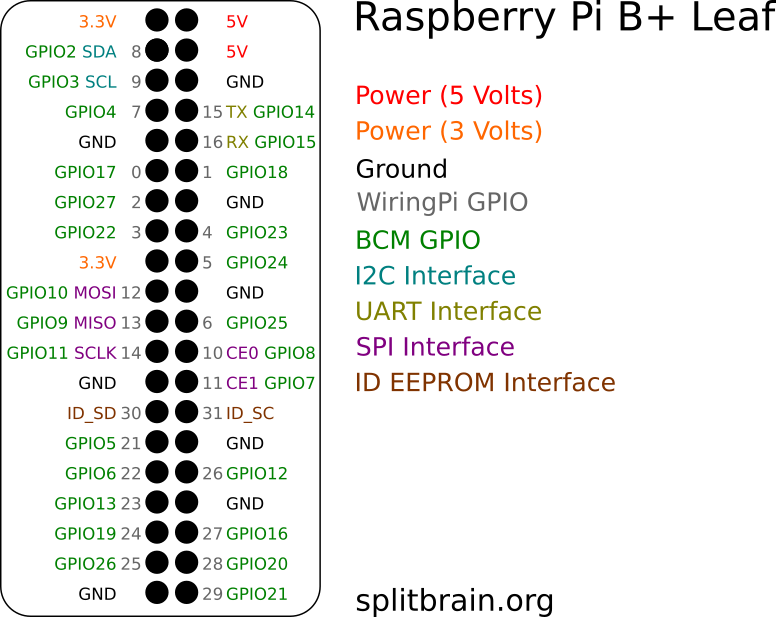
\includegraphics[width=0.7\textwidth,keepaspectratio]{img/pinout.png}
\item
  Interactivo: \url{https://pinout.xyz/pinout/pin33_gpio13}\\
\item
  Uso Básico (esto lo vamos a usar para el \textbf{microfono}):\\
  \url{https://sourceforge.net/p/raspberry-gpio-python/wiki/BasicUsage/}\\
  \url{https://www.raspberrypi.org/documentation/usage/gpio/}\\
  \begin{Verbatim}[breaklines=true, breakanywhere=true]
import RPi.GPIO as GPIO

GPIO.setmode(GPIO.BOARD)
  # or
GPIO.setmode(GPIO.BCM)

GPIO.setup(channel, GPIO.IN)

# Read
GPIO.input(channel)

# Set
GPIO.output(channel, state)

# Poll
if GPIO.input(channel):
    print('Input was HIGH')
else:
    print('Input was LOW')

# To wait for a button press by polling in a loop:
while GPIO.input(channel) == GPIO.LOW:
    time.sleep(0.01)  # wait 10 ms to give CPU chance to do other things

# To clean up at the end of your script:
GPIO.cleanup()
\end{Verbatim}
\end{itemize}

\subsubsection{Para el \textbf{sensor} de temp y humedad:}\label{para-el-sensor-de-temp-y-humedad}

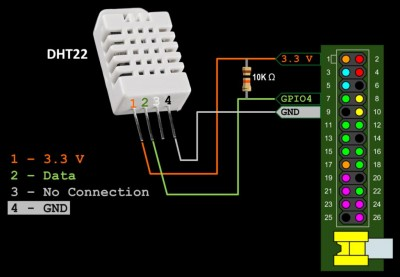
\includegraphics[width=0.7\textwidth,keepaspectratio]{img/sensor.jpg}

\url{https://github.com/adafruit/Adafruit_Python_DHT/blob/master/examples/simpletest.py}\\
\begin{minted}{python}
import Adafruit_DHT
sensor = Adafruit_DHT.DHT22
pin = 23

hum, temp = Adafruit_DHT.read_retry(sensor, pin)
\end{minted}

\subsubsection{Para mostrar la info en las \textbf{matrices de
LED}:}\label{para-mostrar-la-info-en-las-matrices-de-led}

\url{https://luma-led-matrix.readthedocs.io/en/latest/python-usage.html\#x8-led-matrices}\\
\url{https://github.com/rm-hull/luma.examples}\\
\begin{minted}{python}
from luma.core.interface.serial import spi, noop
from luma.led_matrix.device import max7219
from luma.core.render import canvas
from luma.core.legacy import text, show_message
from luma.core.legacy.font import proportional, CP437_FONT, TINY_FONT, SINCLAIR_FONT, LCD_FONT
from luma.core.virtual import viewport

serial = spi(port=0, device=0, gpio=noop())
device = max7219(serial, cascaded=2, block_orientation=-90)
device.contrast(0x05)
msg = 'asd'
# para mostrar un mensage que vaya pasando usar show_message: 
show_message(device, msg, fill="white", font=proportional(LCD_FONT), scroll_delay=0.05)

# para mostrar un mensaje estático usar draw y time para ir actualizándolo:
while True: # o import repeat y repeat(None). 
    time.sleep(1)
     msg = time.asctime()
     msg= time.strftime("%H%M")
     with canvas(device) as draw:
         text(draw, (1, 0), msg, fill="white")
    time.sleep(2)
    pass # ???
\end{minted}
\begin{itemize}
\itemsep1pt\parskip0pt\parsep0pt
\item
  para dibujar en las celdas y obtener el codigo:\\
  \url{http://dotmatrixtool.com/}
\end{itemize}

\subsection{Para \emph{emular}:}\label{emu}

Primero instalamos
\href{https://luma-emulator.readthedocs.io/en/latest/index.html}{Luma.emulation}

\begin{Verbatim}[breaklines=true, breakanywhere=true]
$ sudo apt install python-dev python-pip build-essential
$ sudo apt install libsdl-dev libportmidi-dev libsdl-ttf2.0-dev libsdl-mixer1.2-dev libsdl-image1.2-dev
$ sudo pip install --upgrade luma.emulator
\end{Verbatim}

(recordar hacer lo mismo con \textbf{python3} y \textbf{pip3})

Hay que correr los archivos con unos parámetros especiales. Los más
importantes son:

\begin{Verbatim}[breaklines=true, breakanywhere=true]
   --display DISPLAY, -d DISPLAY
                        Display type, supports real devices or emulators.
                        Allowed values are: ssd1306, ssd1309, ssd1322,
                        ssd1325, ssd1327, ssd1331, ssd1351, sh1106, pcd8544,
                        st7735, ht1621, uc1701x, st7567, max7219, ws2812,
                        neopixel, neosegment, apa102, capture, gifanim,
                        pygame, asciiart, asciiblock (default: ssd1306)
\end{Verbatim}

De estas opciones notar:

\begin{itemize}
\itemsep1pt\parskip0pt\parsep0pt
\item
  \textbf{max7219}: Este es cuando tengamos el dispositivo real.
\item
  \textbf{capture}: Este saca una instantanea de lo que mostraría el display y lo guarda como png.
\item
  \textbf{gifanim}: Este es como capture pero guarda un gif animado.
\item
  \textbf{pygame}: Este muestra el output en una ventana en tiempo real
\end{itemize}

Seguimos con los parámetros restantes

\begin{Verbatim}[breaklines=true, breakanywhere=true]
   --width WIDTH         Width of the device in pixels (default: 128)
   
   --height HEIGHT       Height of the device in pixels (default: 64)
   
   --rotate ROTATION, -r ROTATION
                     Rotation factor. Allowed values are: 0, 1, 2, 3
                     (default: 0)
   --transform TRANSFORM
                     Scaling transform to apply (emulator only). Allowed
                     values are: identity, led_matrix, none, scale2x,
                     seven_segment, smoothscale (default: scale2x)
    --scale SCALE         Scaling factor to apply (emulator only) (default: 2)
\end{Verbatim}

\subsubsection{Por ejemplo, para simular dos módulos de 8x8 en matriz de
led en tiempo
real:}\label{por-ejemplo-para-simular-dos-modulos-de-8x8-en-matriz-de-led-en-tiempo-real}

El código hay que cambiarlo un poco:
\begin{minted}{python}
# from luma.core.interface.serial import spi, noop
# from luma.led_matrix.device import max7219
from luma.core.legacy import text, show_message
from luma.core.legacy.font import proportional, CP437_FONT, TINY_FONT, SINCLAIR_FONT, LCD_FONT
from demo_opts import get_device

# comentar las lineas:
# serial = spi(port=0, device=0, gpio=noop())
# device = max7219(serial, cascaded=2, block_orientation=-90)

device = get_device()

msg = 'Aguante Python y la UNLP 2k19'
show_message(device, msg, fill="white", font=proportional(LCD_FONT), scroll_delay=0.05)
\end{minted}

Y ejecutarlo con los parámetros:
\begin{Verbatim}[breaklines=true, breakanywhere=true]
$ python luma.examples/examples/archivito.py --display pygame --transform led_matrix --width 16 --height 8
\end{Verbatim}
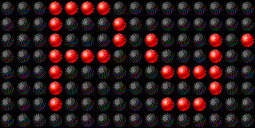
\includegraphics[width=0.4\textwidth,keepaspectratio]{img/gif.png}

\textbar{} \emph{Nota}: ya que hay que usar las librerías demo lo mas
facil es meter el archivo en la carpeta \emph{luma.examples/examples}
que se creó cuando clonamos el git \textbar{}
